\title{Master Project - Real Time Rendering of skeletal structures - Notes on Implicit Surfaces Raytracing}
\author{
        %\large
        \textsc{Olivier Rouiller - s090842}
        \mbox{}\\ %
        Department of Informatics and Mathematical Modelling\\
        Technical University of Denemark\\
        \mbox{}\\ %
}
\date{\today}
\documentclass[11pt]{article}
%\documentclass{acmconf}

\usepackage[paper=a4paper,dvips,top=1.5cm,left=1.5cm,right=1.5cm,
    foot=1cm,bottom=1.5cm]{geometry}

\usepackage{times}
%\usepackage{graphicx}
\usepackage[fleqn]{amsmath}
\usepackage{amsfonts}
\usepackage{amssymb}
\usepackage{amsthm}
\usepackage{amsopn}
\usepackage{xspace}
\usepackage{array}
\usepackage{epsfig}

\numberwithin{figure}{section}

\newcommand\CC{\Lang{\mbox{C++}}\xspace}
\newcommand\Lang[1]{\textsc{#1}}
\newcommand{\kw}[1]{\texttt{\textbf{#1}}}
\newcommand{\cd}[1]{\texttt{#1}}

\newcommand\Naturals{\ensuremath{\mathbb{N}}\xspace}
\newcommand\Integers{\ensuremath{\mathbb{Z}}\xspace}
\newcommand\Rationals{\ensuremath{\mathbb{Q}}\xspace}
\newcommand\Reals{\ensuremath{\mathbb{R}}\xspace}
\newcommand\Complex{\ensuremath{\mathbb{C}}\xspace}

\newcommand\norm[1]{\ensuremath{\lVert#1\rVert}}
\newcommand\abs[1]{\ensuremath{\lvert#1\rvert}}
\newcommand\ceil[1]{\ensuremath{\lceil#1\rceil}}
\newcommand\floor[1]{\ensuremath{\lfloor#1\rfloor}}
\newcommand\set[1]{\ensuremath{\{#1\}}}
\newcommand\angular[1]{\ensuremath{\langle#1\rangle}}

\newcommand\Norm[1]{\ensuremath{\left\lVert#1\right\rVert}}
\newcommand\Abs[1]{\ensuremath{\left\lvert#1\right\rvert}}
\newcommand\Ceil[1]{\ensuremath{\left\lceil#1\right\rceil}}
\newcommand\Floor[1]{\ensuremath{\left\lfloor#1\right\rfloor}}
\newcommand\Set[1]{\ensuremath{\left\{#1\right\}}}
\newcommand\Angular[1]{\ensuremath{\left\langle#1\right\rangle}}

\newcommand{\LOOM}{\ensuremath{\cal{LOOM}}\xspace}
\newcommand{\PolyTOIL}{\textbf{PolyTOIL}\xspace}

\newtheorem{theorem}{Theorem}[section]
\newtheorem{definition}[theorem]{Definition}
\newtheorem{lemma}[theorem]{Lemma}
\newtheorem{corollary}[theorem]{Corollary}
\newtheorem{fact}[theorem]{Fact}
\newtheorem{example}[theorem]{Example}

\newcommand\Cls[1]{\textsf{#1}}
\newcommand\Fig[1]{Figure~\ref{Figure:#1}}

\usepackage{labels} %
\usepackage{equation}
\usepackage{prog2tex}

\newenvironment{excerpt}{\begin{quote}\begin{minipage}\textwidth}{\end{minipage}\end{quote}}

\setcounter{topnumber}{0}
\setcounter{bottomnumber}{0}
\setcounter{totalnumber}{20}
\renewcommand{\textfraction}{0.01}

\begin{document}

\maketitle

\Section[simple]{Metaballs}

\begin{figure}[!h!]
\centering
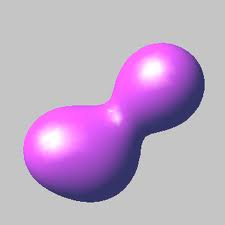
\includegraphics[scale=0.5]{../pictures/meta.jpg}
\caption{MetaBalls}
\label{bilb}
\end{figure}

Metaball defined by $p_i, R_i, f_i, such as, f_i(\|x-p_i\|)=0,\|x-p_i\|<R_i$.
Interested in the surface defined by $f(x)=sigma( q_i f_i(\|x-p_i\|)  ) - T = 0$.
First model Blinn's blob $f_i$ Gaussian function, other with compact support, piecewise quadratic, quartic, degree-six polynomials.

Method to taytrace, solve $f(x)=0$ along the ray. Example solve methods Bezier clipping, piecewise cubic Hermite polynomials.

\Section[simple]{Metaballs Ray Casting on the GPU}

Real-Time GPU Rendering of Piecewise Algebraic Surfaces [BLINN], raytraces algebraic surfacesdefined by Bezier tetrahedra.
GPU-based Fast Ray Casting for a Large Number of Metaballs, Yoshihiro Kanamori, Zoltan Szego and Tomoyuki Nishita, converts metaballs to this class of surface, Bezier clipping.

Root finding regula falsi method

\Section[simple]{Ray tracing experiments}
\subsection{sphere raytracing}
Draw a unit cube centred at the origin, pass camera position to shader, save world position (in this case just gl_Vertex) to the fragment shader.
In the fragment shader construct ray : rayDir = normalize( worldPos - cameraPos );
raytrace from the world position and stop when found a point inside.

Problems with shading, mess up with space.

Result see figs.

Question world space or screen space to construct the rays? at some point needs inverse transform.
Probably better to use a view facing quad.

\subsection{one metaball raytracing}

improved rootfinding by checking sign alternance.
used quadratic metaball function with threshold.


%\bibliography{main,practice,book,crossref}

%\bibliographystyle{abbrv}
\end{document}
